\documentclass[a4paper,12pt,dvipdfmx]{report}

%%%% lib-sty
%% package足りない人はREADME見てください
\usepackage[dvipdfmx]{graphicx}
\usepackage[table,xcdraw]{xcolor}
\usepackage{cite}
\usepackage[numbers,sort&compress]{natbib}% 文献参照の様式を拡張
\usepackage{algorithm, algpseudocode} % アルゴリズム書く人用
\usepackage{mathptmx}
\usepackage{multirow}
\usepackage{bm}
\usepackage{amsmath}
\usepackage{xparse}
\usepackage{caption}
\usepackage{latexsym}
%%% site-sty

%%% original
\usepackage{sty/NGC}

\title{Presentation Training System \\Based On Imitating Past Famous Speech}
\author{SHI Yuhua}
\stdnum{6612160065-0}
\date{\today}
% \date{2016 年 2 月 8 日}

%%%%%%%%%%%%%%%%%%%%%%%%% 本文 %%%%%%%%%%%%%%%%%%%%%%%%%%%
\begin{document}
\baselineskip 1.9zw
\maketitle


\newpage
\thispagestyle{empty}
\pagenumbering{roman}
\setcounter{page}{1}
\chapter*{Abstract}
\par Conference presentation is a non-trivial task since it is affected by both presentation content and nonverbal behaviors. To improve presentation ability, we propose a training method based on imitating the famous past speech. Trainees imitate past famous speech by watching recorded videos, then the proposed system matches they trainees' and the orator's motion data and gives real-time visual feedback on how well they imitate the orators' speech. We employed the OpenPose Library to extract orators' motion data from past famous speech 2D video. During training, the system captures trainee's motion in real-time using the Kinect, then calculate the cosine similarity of adjacent limbs to get the similarity of the trainees' and orator's motion data.  
\par In this paper, we evaluate the effectiveness of our motion data matching algorithm and as well as the system effectiveness. We conducted two experiments to verify the effectiveness of our algorithm and our proposed system. The first experiment results show that the proposed algorithm is able to match the trainee’s motion and the orator's motion in the past famous speech. In our second experiment, we made a A/B test to evaluate the effectiveness of the proposed system. According to the results, we can find that the trainee perform better after training using our proposed system. Notably, the trainees make more gestures and more suitable pauses during the presentation.  

\newpage
\tableofcontents
\listoffigures
\listoftables

\newpage
\pagenumbering{arabic}
\chapter{Introduction}
\par The presentation is the art of persuasion, It plays a significant role in our society and has the tremendous impact on the success of everyone \cite{seiler2002communication}. The presentation commonly used to communicate the presenter's ideas to the listener. However, giving a presentation successfully like John F. Kennedy or Steven Jobs is not a simple thing. A great preparation not only contains verbal style but also needs various nonverbal behaviors. On one hand, the content of a preparation must be clear, vivid and appropriate\cite{rodman1996style}. On the other hand, the significant component of a presentation lies upon nonverbal cues which have the power to change the meaning assigned to spoken words\cite{seiler2002communication}. 
\par Nonverbal behaviors of public speakers are expressed via several channels such as voice, gesture and facial expression. They have been proven to have a more significant influence than verbal cues. According to Argyle nonverbal messages are thirteen to fourteen times more powerful than verbal ones\cite{argyle1971communication}. Likewise, Arcy showed that the audience receives more than half of information from nonverbal behaviors\cite{d1998communicating}. The study of Seiler\cite{seiler2002communication}shows the fact that most people unconsciously believe more in nonverbal behaviors than verbal cues.
\par Unfortunately, it's hard to practice to express the effective nonverbal behaviors because they are mostly expressed subconsciously. To achieve the learning results, trainees must be provided with appropriate feedbacks from human advisors, but it is costly and not always available. According to Seiler \cite{seiler2002communication}, imitation is a kind of effective method to help the trainee to refine their nonverbal behaviors. Imitating those past famous speakers' gesture, sound or enunciation to learn what they're doing right, and then try to make it your own as Pablo Picasso said \emph{`` Good Artists Copy. Great Artists Steal "}. It is a great learning experience and can stretch trainees' abilities.
% because it requires certain skills\cite{rosenberg2005acoustic}. One aspect is the preparation of the presentation draft in advance, it can be relatively easily refined by revising the presentation draft many times by theirselves. Many books and tutorials have been written through training. The other is the way the orator delivers the presentation to others. It is difficult to be refined because they need to practice for many times and get some advice from the professionals to know their shortcomings, and it will cost a lot of time and money. 

\par In parallel, the role of nonverbal behaviors in computing is becoming increasingly recognized by the development of the emerging fields, such as social signal processing and affective computing. Such as \cite{Chen,cao2017realtime,Fang2016,Papandreou2017,He2017}, those Deep Learning library can extract user's body key point with high accuracy. Therefore, computers have been equipped with the abilities to decode the complexity of humans nonverbal channels. 

\par Many papers discussed some approaches toward the automatic recognition of nonverbal from trainees. However these approaches all defined some exact rules in advance to give a score of the presentation, but few have focused on imitating past famous speech to refine their nonverbal behaviors. 
 
\par In this paper, we propose a presentation training system that allows the trainee to imitate past famous speech to improve their nonverbal behaviors. Nonverbal behaviors include many aspects, and we choose to analyze the gesture of orators as the nonverbal behavior in this paper. In advance, we employed OpenPose library\cite{cao2017realtime} to extract orators' motion data from past famous speech 2D video. While training, the system capture the trainee's motion in real-time using Microsoft Kinect. We choose the cosine similarity of adjacent limbs as the feature to calculate the score that shows the similarity of the trainees' motion and the motion of extracted orators. The trainees will also wear an HMD that show a virtual hall and some virtual audience. The audience will perform some actions according to the score.
\begin{figure}[htbp]
\centering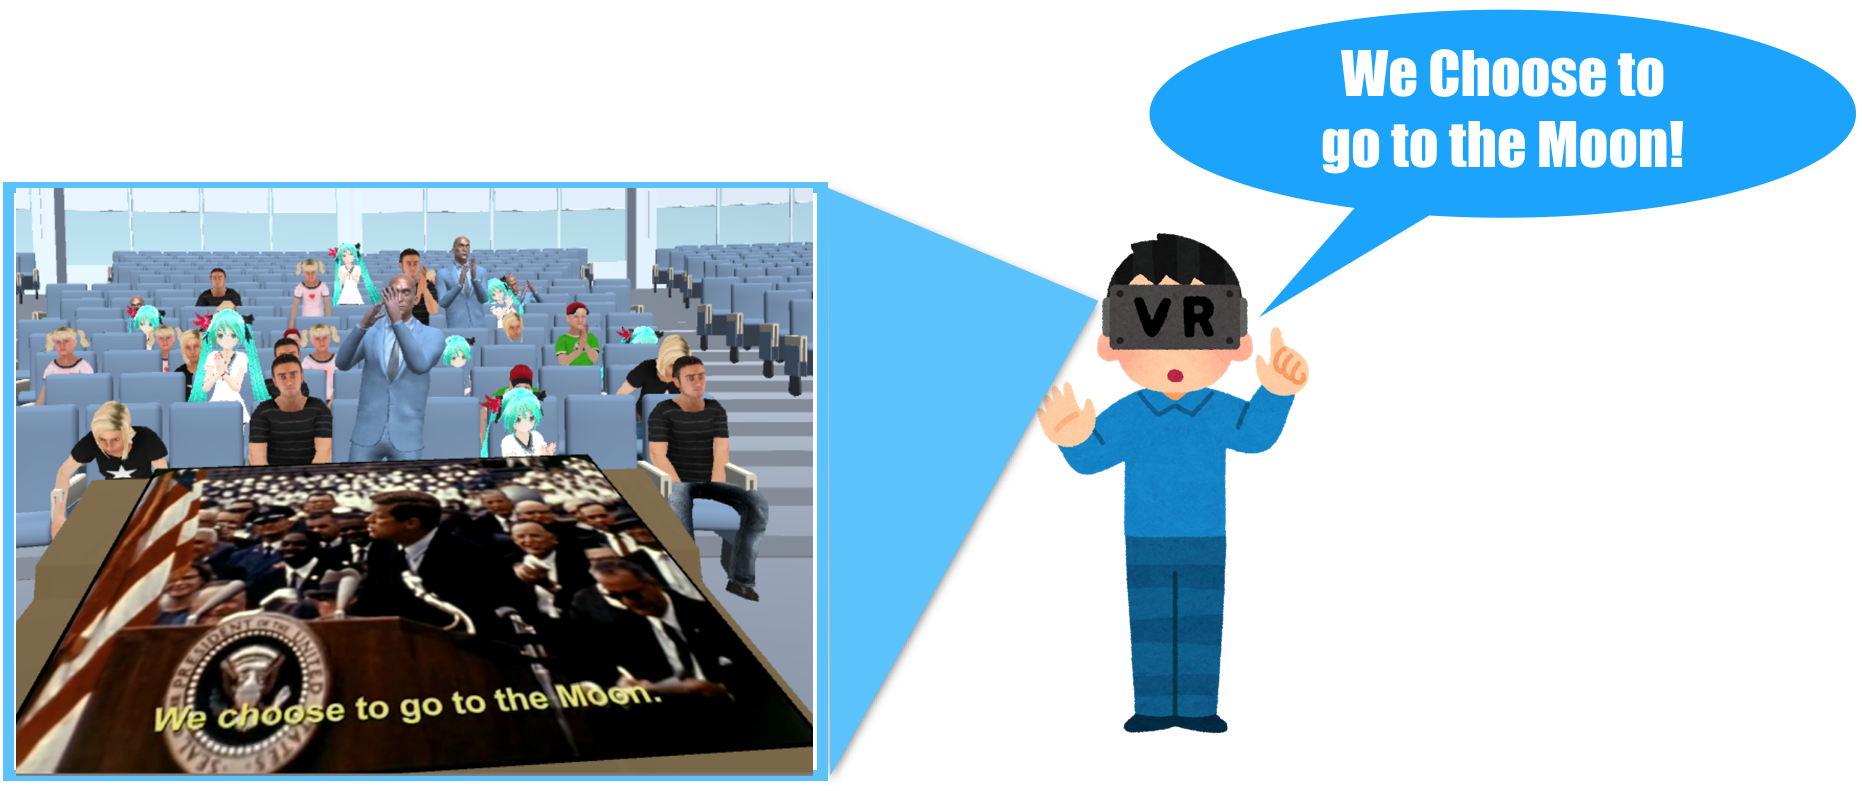
\includegraphics[scale=0.225]{./img/Introduction.png}
\caption{System Introduction}\label{fig:System Introduction}
\end{figure}

\par The rest of this paper is organized as follows. First we will introduce some existing presentation training method and proposed solution in the chapter 2. Then we will introduce the preparation about OpenPose, Kinect and the Evaluation of presentation in the chapter3. The chapter 4 describes our proposed system in detail. In the chapter 5, we will evaluate the system and discuss the results. The last chapter is for conclusions and future works.

\chapter[Related Work]{Related Work}
\par Presentation skills give us the power to change the world. Great presenters instill trust, engage our minds and hearts, deliver ideas and information, and inspire and captivate us.

\par In this paper, we propose a presentation training system that allows trainees to imitate past famous speech to improve their nonverbal behaviors. Many papers discussed some approaches toward the automatic recognition of nonverbal from trainees. However these approaches all defined some exact rules in advance to give a score of the presentation, but few have focused on imitating past famous speech to refine their nonverbal behaviors. Some researches analyze some visual and vocal channels of trainees, thus can provide information about their presentations. For example, the system in Pfister was originated from a vocal emotion detection module \cite{pfister2011real}. It was similar to the approach of Silverstein \cite{Silverstein2006}, which was built solely on vocal cues, by analyzing the voice such as pitch or tempo. The Hincks's system measured the changes in vocal pitch, and then give visual feedback to promote pitch variation by relying on the importance of pitch variance in oral presentations \cite{hincks2009promoting}.
\par On the other hand, some include nonverbal behaviors in the analysis. Gao introduced the method based only on visual information \cite{Gao}. In contrast, Kurihara added face position and orientation as the approximation of eye contact, together with pitch, speaking rate, utterance and filled pauses \cite{Kurihara2007}. Hoque proposed an automated conversation coach to help trainees improve their interview skills by recognizing their motion and facial expression \cite{Kurihara2007}.
\par We will introduce the detail about Kurihara's research \cite{Kurihara2007} in section 2.1 and Nguyen's research \cite{nguyen2015intelligent} in section 2.2. 

\section{Presentation Sensei}
\label{sensei}
\par In Kurihara's paper, they present a presentation training system that observes a presentation rehearsal and provides recommendations for improving the delivery of the presentation, such as to speak more slowly and to keep eye contact with the audience (Figure \ref{fig:sensei}). Kurihara intentionally focuses on the basic behavior patterns because high-level semantics is very difficult to analyze by computers in contrast to basic behavior patterns. Kurihara's goal is to help people improve their base-line presentation skills by reducing inappropriate behavior such as using many fillers (e.g., “er”) or continuously looking down at the script.

\begin{figure}[htbp]
  \centering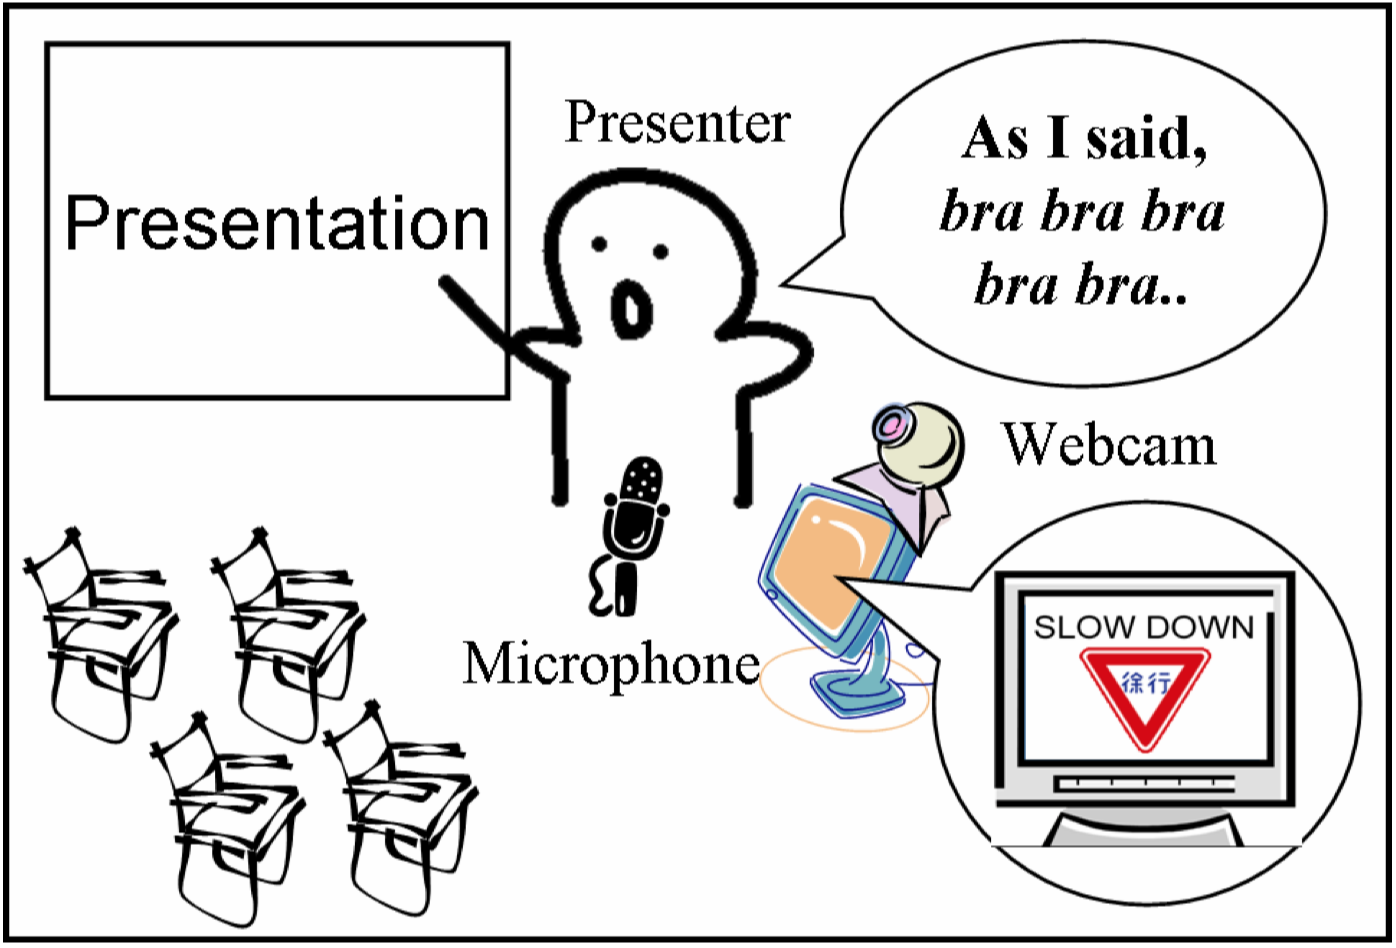
\includegraphics[width=0.8\textwidth]{./img/sensei.png}
  \caption[Presentation sensei system]{Presentation sensei system \cite{Kurihara2007}}
  \label{fig:sensei}
\end{figure}

\par In this work, Kurihara focus on the following five aspects of presentation delivery.
\begin{itemize}
  \item The speaking rate should not be too fast.
  \item The speech should not be monotonous.
  \item The speech should not contain too many fillers.
  \item The speaker should look at the audience and avoid continuously looking down at a script or a screen.
  \item The speaker should finish the presentation within a certain time limit.
\end{itemize}

\par Kurihara selected these because they are emphasized in the existing literature, and they can be detected to some extent using current speech processing and image processing technologies. The Presentation Sensei system visualizes the analysis result in real time communicating with a presentation tool. It can give the presenter both instant “online” feedback and post “offline” feedback for improvements. The online feedback function shows the analysis result in real-time. When the system detects some inappropriate behavior, it alerts the presenter by showing a visual signal (Figure \ref{fig:onlinefeedback}). The offline feedback function shows the visual summaries of the indices for the presenter’s self-examinations (Figure \ref{fig:offlinefeedback}).

\begin{figure}[htbp]
  \centering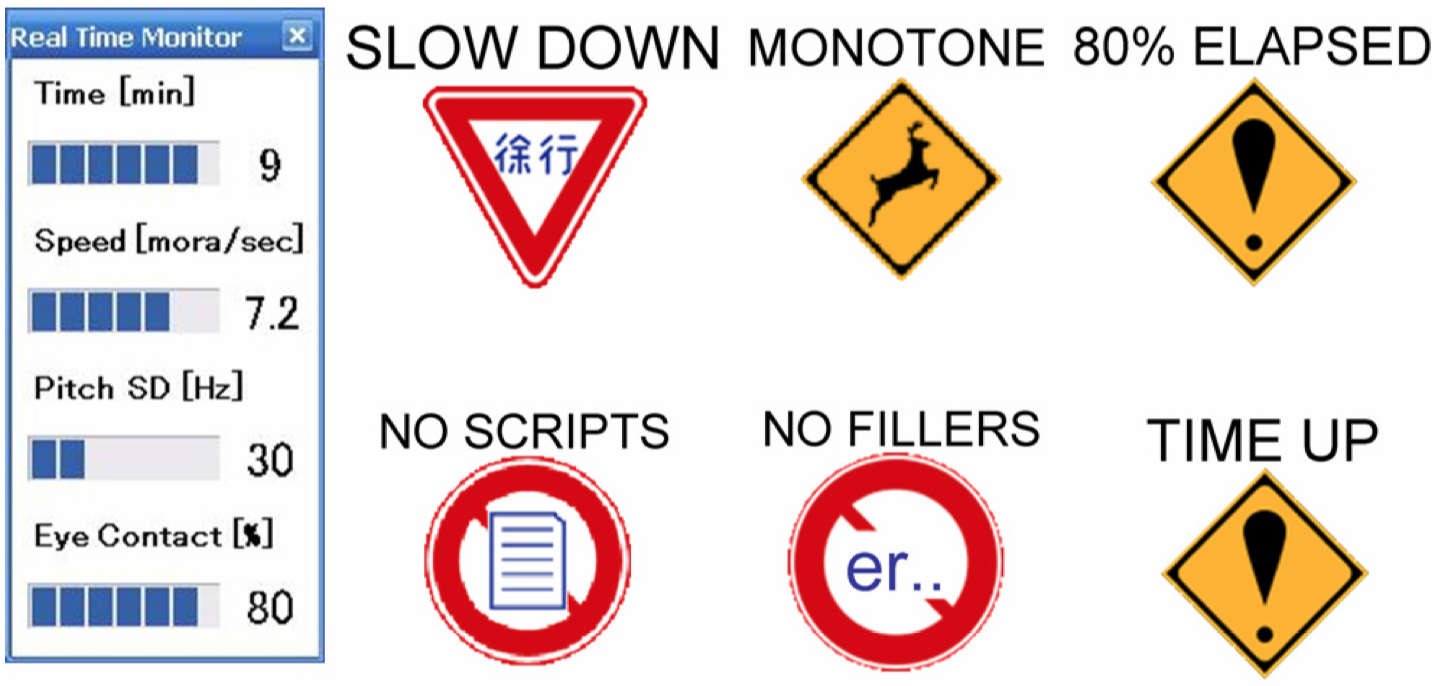
\includegraphics[width=0.5\textwidth]{./img/onlinefeedback.png}
  \caption[Online feedback of presentation sensei]{Online feedback. (Left) Real time monitor. (Trafic signals) Visual Alerts.\cite{Kurihara2007}}\label{fig:onlinefeedback}
\end{figure}

\begin{figure}[htbp]
  \centering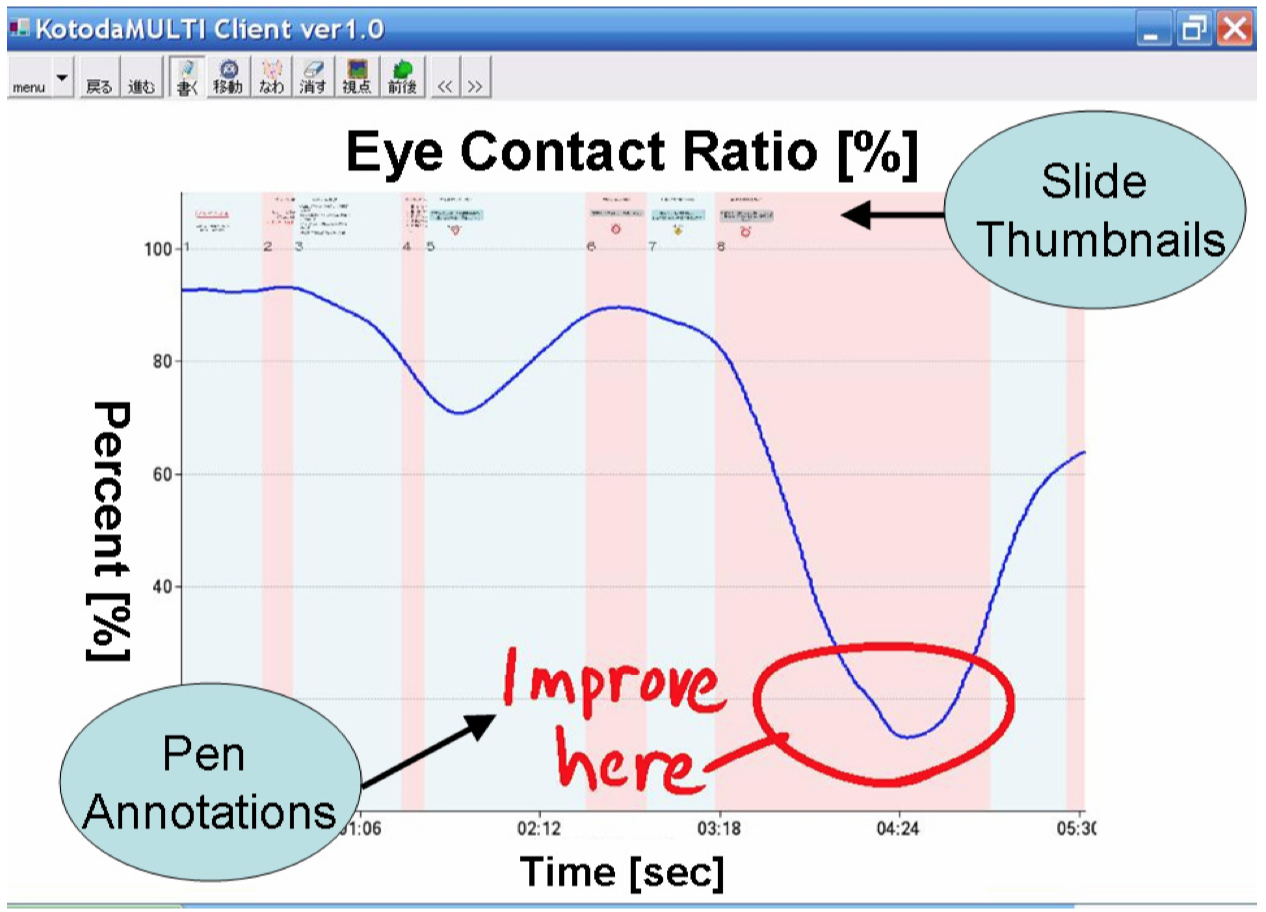
\includegraphics[width=0.5\textwidth]{./img/offlinefeedback.png}
  \caption[Offline feedback of presentation sensei]{Offline feedback. An example of the generated charts\cite{Kurihara2007}.}\label{fig:offlinefeedback}
\end{figure}

\par It is often difficult to make speech processing and image processing work robustly in adverse environments. One advantage of Kurihara's target application domain, personal presentation rehearsal, is that we can relatively freely configure the environment. It is realistic to rehearse in a silent room with no visual obstacles, where these technologies perform the best. This feature makes the Presentation Sensei system a highly practical application even with imperfect recognition technologies \cite{Kurihara2007}.
\par Kurihara's system is unique in that, while general multimodal systems help the user to control computers, it tries to help computers guide humans. This way of using a computer is relatively new. Heer et al. \cite{Heer} investigated the design guidelines for this sort of systems and also introduced an experimental media capture system that acts as a film director. 
\subsection*{System Configuration}
\par The Presentation Sensei system consists of several modules connected by a network (Figure \ref{fig:senseisystem}). The audio analysis module continuously analyses the input signal from a microphone and provides the integration module with the results of the utterance duration detection, pitch (F0) detection, and filled pause detection. The speech recognition module also continuously provides the integration module with the mora-based speech recognition results. The image processing module continuously analyzes the input from a webcam and provides the integration module with the result of the face position/orientation detection. The integration module integrates all the provided information and gives feedback to the presenter using various monitors. These modules can be distributed over a local network for the load sharing purpose, and they communicate with each other via RVCP protocol \cite{Goto2001}. The system can also be connected to a third party presentation tool to achieve synchronization. Kurihara currently connects their system to an in-house presentation program to receive timing information and thumbnail images of slides.

\munepsfig[width=0.8\textwidth]{senseisystem}[System configuration of presentation sensei]{System configuration of presentation sensei \cite{Kurihara2007}}

\section{Intelligent Presentation Skills Trainer}
\par Nguyen's research developed a tutoring system for public speaking, which assesses presentations based solely on the visual behaviors of presenters. Firstly, an empirical study was performed to investigate on the nonverbal cues that impact a presentation, serving as the ground truth. Next, a Microsoft Kinect was implemented for capturing skeletal representations of the presenters' body as input data for the analysis. The recognition process can detect if the behaviors appeared in real-time. Multi-class support vector machine was used to classify the quality of presentations into a four-degree scale with the recognition rate of 73.9\% on a training/test database that includes 76 presentations. For the feedback, the system allows presenters to review their presentation, together with the analysis results. They also developed a simulated conference room as the real-time feedback mechanism.
\subsection*{Automatic Feedback System}
\par In order to support presenters with an effective solution that can help them self-practice even at home, Nguyen aimed to implement the system with the following functions: (1)Automatic analyzes presenters performance; (2)Provides immediate feedback during the presentation; (3)Provides overall analysis about the whole presentation; (4)Lets users review their performance together with the analyzed results, thus allows them to keep track of their practicing progress. To achieve these purposes, they set up a Microsoft Kinect to extract body's skeletal representation as input for the analysis task. In parallel, a regular camera or webcam is positioned to simulate the audience's point of view. The automatic analysis, as well as recording,  is processed in real-time using a regular PC. The result is visualized on the PC or an external screen/projector (Figure \ref{fig:nguyensystem}). Users also have the chance to review their presentations, together with in-depth analysis of nonverbal cues in the end.
\munepsfig[width=0.5\textwidth]{nguyensystem}[Setup of the Nguyen's system]{Setup of the Nguyen's system \cite{nguyen2015intelligent}}

\subsection*{The Two Methods of Giving Feedbacks}
\par Nguyen's system provides two ways of delivering feedback to the audience \cite{nguyen2015intelligent}. The first one shows users their recorded presentation, the appearances of each behavior and results on the four nonverbal aspects, plus the overall result. In parallel, with the purpose to give presenters the helpful feedbacks, also aim to provide them the experience as presenting for the real audience, Nguyen developed a virtual conference room as one method to deliver feedbacks. The environment was built using the Unity3D engine, simulates the classroom that we collected data for observation. Avatars can perform several animations that may bring either a positive or negative feeling for presenters. These animation clips are sorted based on the increase of negative feeling: (1) Nodding; (2) Sitting still; (3) Sleeping; (4) Yawning.


\munepsfig[width=0.8\textwidth]{feedback_n}[The simulated conference room]{The simulated conference room \cite{nguyen2015intelligent}}


\chapter{Preparation}
本章では, 本論文で提案する○○手法の基礎となるSPFDによる論理関数の自由度の表現方法について説明する.


\chapter{Proposed Method}
この章がメイン.提案手法について説明する.

ここが短いと卒業(修了)させてもらえないらしい.

アルゴリズムの入れ方のサンプルをAlgorithm~\ref{alg:prop}に貼っときます.
\begin{algorithm}[tbp]
 \caption{Proposed method using CSPF}\label{alg:prop}
 \begin{algorithmic}[1]
  \Require $C$:生成回路となるAQFP論理回路
  \State $C \gets$ RAND-1を用いてAQFP論理回路に変換された入力回路
  \State コメント \Comment{ステップ1}
  \State 行にもラベルを貼れます(参照テスト[\ref{alg:prop:hoge}行目]) \label{alg:prop:hoge}

  \If{あほあほ}
  \State ifはこんな感じ
  \State \Return \True
  \ElsIf{ぼけぼけ}
  \State \Return \False
  \EndIf

  \For{$i=1$ to N}
  \State forはもちろん
  \EndFor

  \ForAll{外部出力リストのゲート\textit{po}}
  \State forallや
  \EndFor

  \Repeat
  \State リピートも使えます
  \State $C$内のそれぞれのゲートの出力論理を計算
  \State OptimizeCircuitUsingCSPF($C$)
  \Until{$C$の構成に変更なし}

  \State \Return $C$
 \end{algorithmic}
\end{algorithm}

\chapter{Evaluation}
本章では,提案した○○手法を○○に適用した実験結果とその考察を示す.

\section{Method}
評価方法が細かい説明が要る場合は,節を分けて方法だけを説明するのもあり.
節を分けるほどでなければ,実験したマシン,環境,などについて1から2段落で説明する.

\section{Results}

結果を表\ref{table:result_bench1}に示す.

表の例:たての罫線(外側)を使わないのが格好いいらしい.

\begin{table}[tbp]
\caption{分析結果1}
\begin{tabular}{l|r|r|r|r} \Hline
 & \multicolumn{1}{l|}{gcc} & \multicolumn{1}{l|}{li} & \multicolumn{1}{l|}{m88ksim} & \multicolumn{1}{l}{go} \\\hline
収束回数 & 4346  & 5930  & 2595  & 3545  \\\hline
総保存命令数 & 50711  & 72519  & 28562  & 81305  \\\hline
再利用可能な総命令数 & 47366  & 59178  & 28277  & 78317  \\\hline
平均再利用可能命令数 & 10.90  & 12.30  & 10.90  & 22.09  \\\hline
保存した命令が一部, 再利用できない回数 & 363  & 1350  & 35  & 349  \\\hline
\end{tabular}
\label{table:result_bench1}
\end{table}


以上の結果より以下のことが言える.
実験結果の後は,考察を分かりやすくまとめる.箇条書きを使ってもよい.

*すぐに導かれる将来の課題はここに書いてしまっても良い.そして,「おわりに」に
再度書いてもOK

\chapter{Conclusion and Future Work}
本研究では,○○という手法において,○○保存する命令を,分岐の信頼性を用いて限定する手法を提案した.
(略)
その結果,再利用できない無駄な命令の保存を,最大で95\%削減することができた.
今後は,さらに○○の部分を改良することにより削減割合をさらに向上させることが課題である.

ここまできたら,力尽きそうですが,力を振り絞って,
\begin{itemize}
\item 本論文の概要と特徴
\item 得られた成果
\item それから得られる最終結論
\item 残された課題
\end{itemize}
は書いてください.

\chapter*{Acknowledgement}
\par 本論文の執筆にあたり、多岐に渡るご指導をしてくださり、私を導いてくださった野間春生教授に深く感謝の言葉を申し上げます。至らぬ私が無事に論文の執筆を終えるができたのは野間春生教授の教えがあったからです。本当にありがとうございます。また、鋭い指摘や温かい助言を下さったLopez Rober Gulliver 准教授に深く感謝の意を述べさせて頂ます。スイカバーを嬉しく召し上がる姿には、心を癒されました。そして同研究室の松村耕平講師と大井翔講師からは、ゼミナールを中心に一歩引いた視点からの意見をいただきました。ありがとうございました。
\par 研究の日々を互いに切磋琢磨し、励まし合いながら過ごした研究室の皆様に輝かしい未来があるようお祈り申し上げます。自らもお忙しいなか、快く実験への協力を承諾いただきました被験者の皆様への恩は一生涯胸に残します。研究のみならず数々の困難を共に乗り越えてきた同級生の方々が, これからも健やかに過ごし、皆様の力を存分に発揮できるような日々を送られますよう心からお祈りいたしま。
\par そして何よりも、この24年間私を育て、支えてくれた両親に心から感謝いたします。


\bibliographystyle{ieeetr}

\bibliography{/Users/shiyuhua/Documents/Reference/MyCollection}
\chapter*{Appendix}

\addcontentsline{toc}{chapter}{Appendix}
\setcounter{figure}{0}    
\renewcommand{\thefigure}{A. \arabic{figure} }
\munepsfig[width=0.65\textwidth]{sa1}[Evaluation sheet of subject A1]{Evaluation sheet of subject A1}
\munepsfig[width=0.7\textwidth]{sa2}[Evaluation sheet of subject A2]{Evaluation sheet of subject A1}
\munepsfig[width=0.7\textwidth]{sa3}[Evaluation sheet of subject A3]{Evaluation sheet of subject A1}
\munepsfig[width=0.7\textwidth]{sa4}[Evaluation sheet of subject A4]{Evaluation sheet of subject A1}
\munepsfig[width=0.7\textwidth]{sa5}[Evaluation sheet of subject A5]{Evaluation sheet of subject A1}
\munepsfig[width=0.7\textwidth]{sb1}[Evaluation sheet of subject B1]{Evaluation sheet of subject A1}
\munepsfig[width=0.7\textwidth]{sb2}[Evaluation sheet of subject B2]{Evaluation sheet of subject A1}
\munepsfig[width=0.7\textwidth]{sb3}[Evaluation sheet of subject B3]{Evaluation sheet of subject A1}
\munepsfig[width=0.7\textwidth]{sb4}[Evaluation sheet of subject B4]{Evaluation sheet of subject A1}
\munepsfig[width=0.7\textwidth]{sb5}[Evaluation sheet of subject B5]{Evaluation sheet of subject A1}


\end{document}
